\section{Methods -- Experiment 2: Importance of Video Elements}
\label{method-2}
Results in the first experiment implied that QV aligned closer to the participant's truthful preferences compared to the Likert scale when choosing among a set of societal issues. To strengthen our results and examine the generalizability of QV, we designed a second experiment with three changes in mind: 1) a change in topic domain, 2) a change in the relationship of items on the survey, 3) a change in the degree of the tangibility of the survey outcome. We describe the goal of these changes below.
% , and 4) a change from between-subject to within-subject study

First, we changed the application domain from public policy to HCI to explore if QV's advantage of better alignment generalizes to a different domain. HCI studies often rely on preference elicitation from users to inform designs and create better user experiences that involve trade-offs. These characteristics made HCI studies an excellent domain to test out QV. 

Second, we changed the \textit{relationships} among items in the survey. This experiment focused on ballot items that represented different \textit{aspects} of the same subject matter that may interact with one another, a typical case in the HCI domain. In the previous experiment, the items were paralleled on the same topic, i.e., different societal causes (items) impacted the society (topic) on their own without influencing each other. To give a simple analogy: the first experiment asks about one's preference among chocolate, strawberry, and vanilla ice cream (paralleled options), whereas the second experiment asks how much one cares about the texture, flavor, and color of ice cream (aspects of the same object that may influence each other). Since the difference in relationships may impact how users make trade-offs, we want to examine if QV also aligns better than Likert in this use case.
% We hypothesize that the latter case is more challenging for the participants to express accurately. Thus, if QV could outperform Likert in such cases, it will broaden the use cases for QV.

Lastly, the second experiment focused on a setting that surveyed matters with a more tangible and immediate outcome to the participants, a common scenario in HCI studies, as opposed to matters with a more abstract and further-in-the-future impact. This difference may also impact the performance of QV and Likert. 
% Our last change made the second experiment a within-subject study to understand how the same individual's expression differs using different survey tools.

We hypothesized that QV would outperform Likert in accurately representing the participants' true preferences in the new setting. To verify our hypothesis, we designed a within-subject study that elicited participants' preferences on different video elements using QV, Likert, and a pricing task. In this section, we first explain how we selected video streaming experience as the HCI study scenario. Then, we demonstrate the experiment workflow accompanied by the interfaces of the experiment. Finally, we explained the analysis approach.

%<---------------------------->%
% HCI Experiment background
%% Video HCI experiments
%% Selection of the five elements and their definitions
%% The goal of this HCI experiment is to find elements that impact participants most.
%<---------------------------->%
 
\subsection{Choice of HCI study}
The selected HCI study scenario needs to align with the three changes specified above. We set out to find a typical use case where UX/UI researchers survey users to understand what features to prioritize. In the end, we decided to use the research scenario of understanding users' preferences among various video and audio elements under network or monetary constraints \cite{molnar2013comedy, oeldorf2012bad}.
% On the one hand, we wanted to avoid creating an entirely new HCI study that required sophisticated verification. On the other hand, reproducing a prior HCI study that used Likert surveys can be costly and difficult because of the limited access to the devices, designs, or interfaces used in the study. Therefore, we developed new research based on prior research but with a new research question and study design to maintain ecological validity.

Research on video and audio elements of video playback from the lens of HCI is relatively mature. Among a variety of topics, understanding how users with bandwidth constraints made trade-offs across multiple videos and audio elements \cite{molnar2013comedy, oeldorf2012bad} is a typical topic to explore which of the $K$ aspects of the same subject should be prioritized under constraints. \textcite{oeldorf2012bad}, for example, conducted a study to examine the differences in participants' perceptions between three video bit rates, three video frame rates, and two audio sampling rates across three types of video content via a 5-point Likert scale. 
% Participants rated the overall quality, video quality, audio quality, and enjoyment level  in each condition. The study derived the conclusions from analyzing the means and standard deviations of the Likert survey results. This HCI experiment is a typical study to explore which one or some of the $K$ elements to prioritize under constraints.
% Researchers provided insights to topics including multi-media conferencing \cite{watson1996evaluating}, video-audio perception \cite{chen2006cognitive, molnar2015assessing}, and, more specifically, trade-offs among various video and audio elements under network or monetary constraints \cite{molnar2013comedy, oeldorf2012bad}. understand how users with bandwidth constraints made trade-offs covering a broad set of elements across multiple videos and audio elements. They 

We proposed a similar user research topic as in \textcite{oeldorf2012bad}'s study. We designed the experiment to answer the following question: ``Given a video with unsatisfying quality, under limited bandwidth, how should the bandwidth be allocated to enhance the five video and audio elements, including motion smoothness \cite{huynh2008temporal}, audio stability \cite{hardman1998successful}, audio quality \cite{knoche2008low}, video resolution \cite{knoche2005can}, and audio-video synchronization \cite{steinmetz1996human}, to obtain an acceptable video streaming experience from the viewers' perspective?'' We selected the five video elements based on prior work. For their detailed definitions, please refer to \Cref{elem_def}. To our knowledge, no prior work has studies the combination of five elements in a single experiment.

Prior work suggested that the type of video affected users' perceptions for video elements. In this experiment, we used a 90-second weather forecast video for the United States. There are two reasons why we chose the weather forecast video. First, the concept of a weather forecast is generic and universal. The terms used in the weather forecast are usually easy to understand. Second, since we are studying both audio and video elements, we wanted a video that conveyed information via both visuals and speech. In a weather forecast video, the meteorologist usually spoke aloud the weather while pointing at visual cues such as icons and numbers.
% There is no prior literature that looked at five combinations in a single experiment and studied them together, to the best of our knowledge. Hence, this is a valid HCI-related research question. We are also aware that these video elements' importance relies heavily on the type of video being served. 
% Video clips such as sports can contain specific jargon, while movie clips can be unfamiliar to some and not to others. a large amount of visualization but also provided information through speech. Drama and talk shows, for example, would lean towards visual elements or audio elements. Finally, visual and audio elements in a weather forecast complement each other. 

In the next section, we describe how we conducted the video elements trade-off experiment to compare the performance between Likert and QV surveys in truthfully reflecting users' preferences across the video/audio elements.
% answering the research question in identifying the video/audio elements that impact participants' streaming experience the most.

\begin{figure}[htpb]
    \centering
    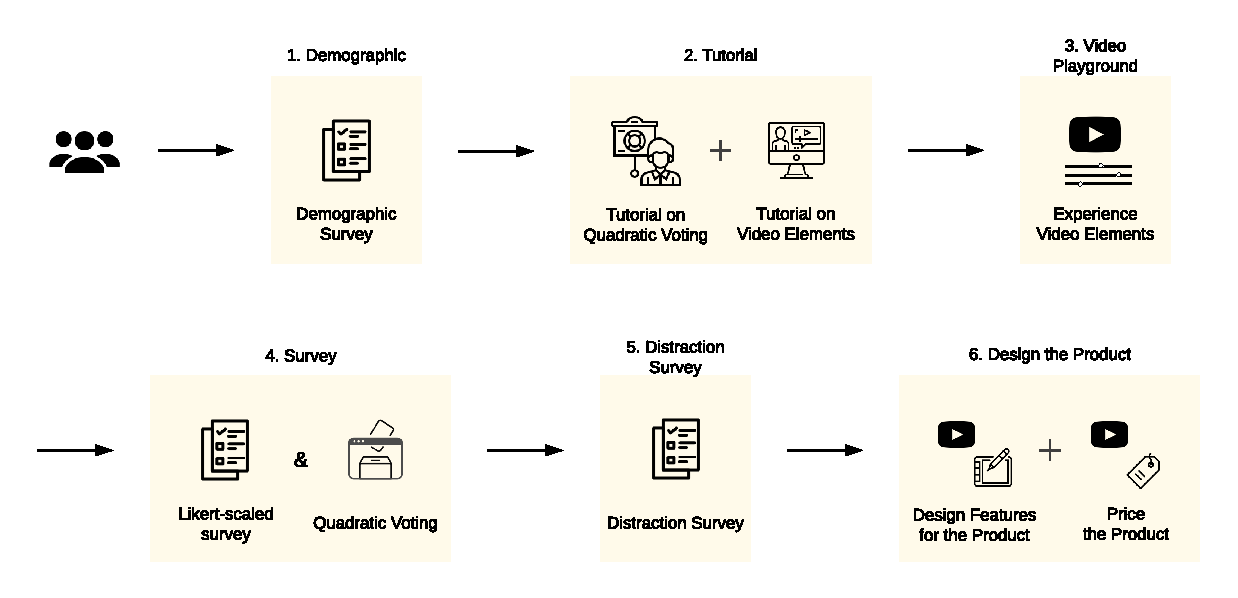
\includegraphics[width=\textwidth, keepaspectratio=true]{content/image/exp2_procedure.pdf}
    \caption{
        We used a within-subject design for experiment two. We randomly assigned participants into two groups: one group would complete the Likert survey first and then quadratic voting; the other group experienced them in a reversed order.
    }
    \label{fig:exp2_flow}
\end{figure}

\subsection{Experimental Flow}

% To compare how well the Likert survey and QV reflect people's underlying preferences, we designed the following experiment. 
We recruited participants through MTurk. Like our first experiment, we used a demographic survey to match the participants' distribution with the U.S. population in age and education. All participants followed six steps, as shown in \Cref{fig:exp2_flow}. The six steps were (1) demographic survey, (2) tutorials and attention checks, (3) a video playground, (4) Likert and QV surveys, (5) a distraction survey, and (6) a design task. The experiment took X minutes to complete on average. Turkers received a compensation of \$6 U.S. dollars if they complete their work and a possible bonus up to \$2 dollars. Now we explain the six steps in detail with the actual study provided as supplementary material.

\subsubsection{Step 1. Demographic}
We greeted participants with a consent form. In the consent form, we told the participants that the study aims to collect how different people think about the importance of the different elements when watching a video. We did not reveal to the participants that this experiment aimed to compare Likert and QV until they completed the survey. Once participants gave their consent, participants would fill out a demographic survey. The demographic survey contained questions identical to the first experiment.

\subsubsection{Step 2. Tutorials and attention checks}
In step two, we provided two tutorials to the participants. All participants would read through a tutorial that defined the five video elements described in the experiment. In this tutorial, for each video element, we showed a pair of videos side-by-side for participants to compare how the same video would differ if a particular element were perfect and when the element is of lousy quality. Once the participants thought they understood the concepts, we asked them to answer five multiple choice questions related to the tutorial concepts. We also included two attention checks to make sure the participant's audio and video worked fine. Participants would be disqualified from the experiment immediately if they answered two or more of the questions incorrectly. This step makes sure participants fully understand the terminology used for the rest of the experiment.

Participants would then move to the tutorial on QV since QV is unpopular among the mass. The tutorial provided a short video explaining QV supplemented with text. Participants were allowed to play with the QV interface similar to Figure \ref{fig:qv_donation} with types of cuisine as the options. Once participants are confident that they understand QV, they need to complete a quiz consisting of five true-false questions and two attention questions. The system would disqualify the participants immediately if they answered two or more of the questions incorrectly.

\begin{figure}[htpb]
    \centering
    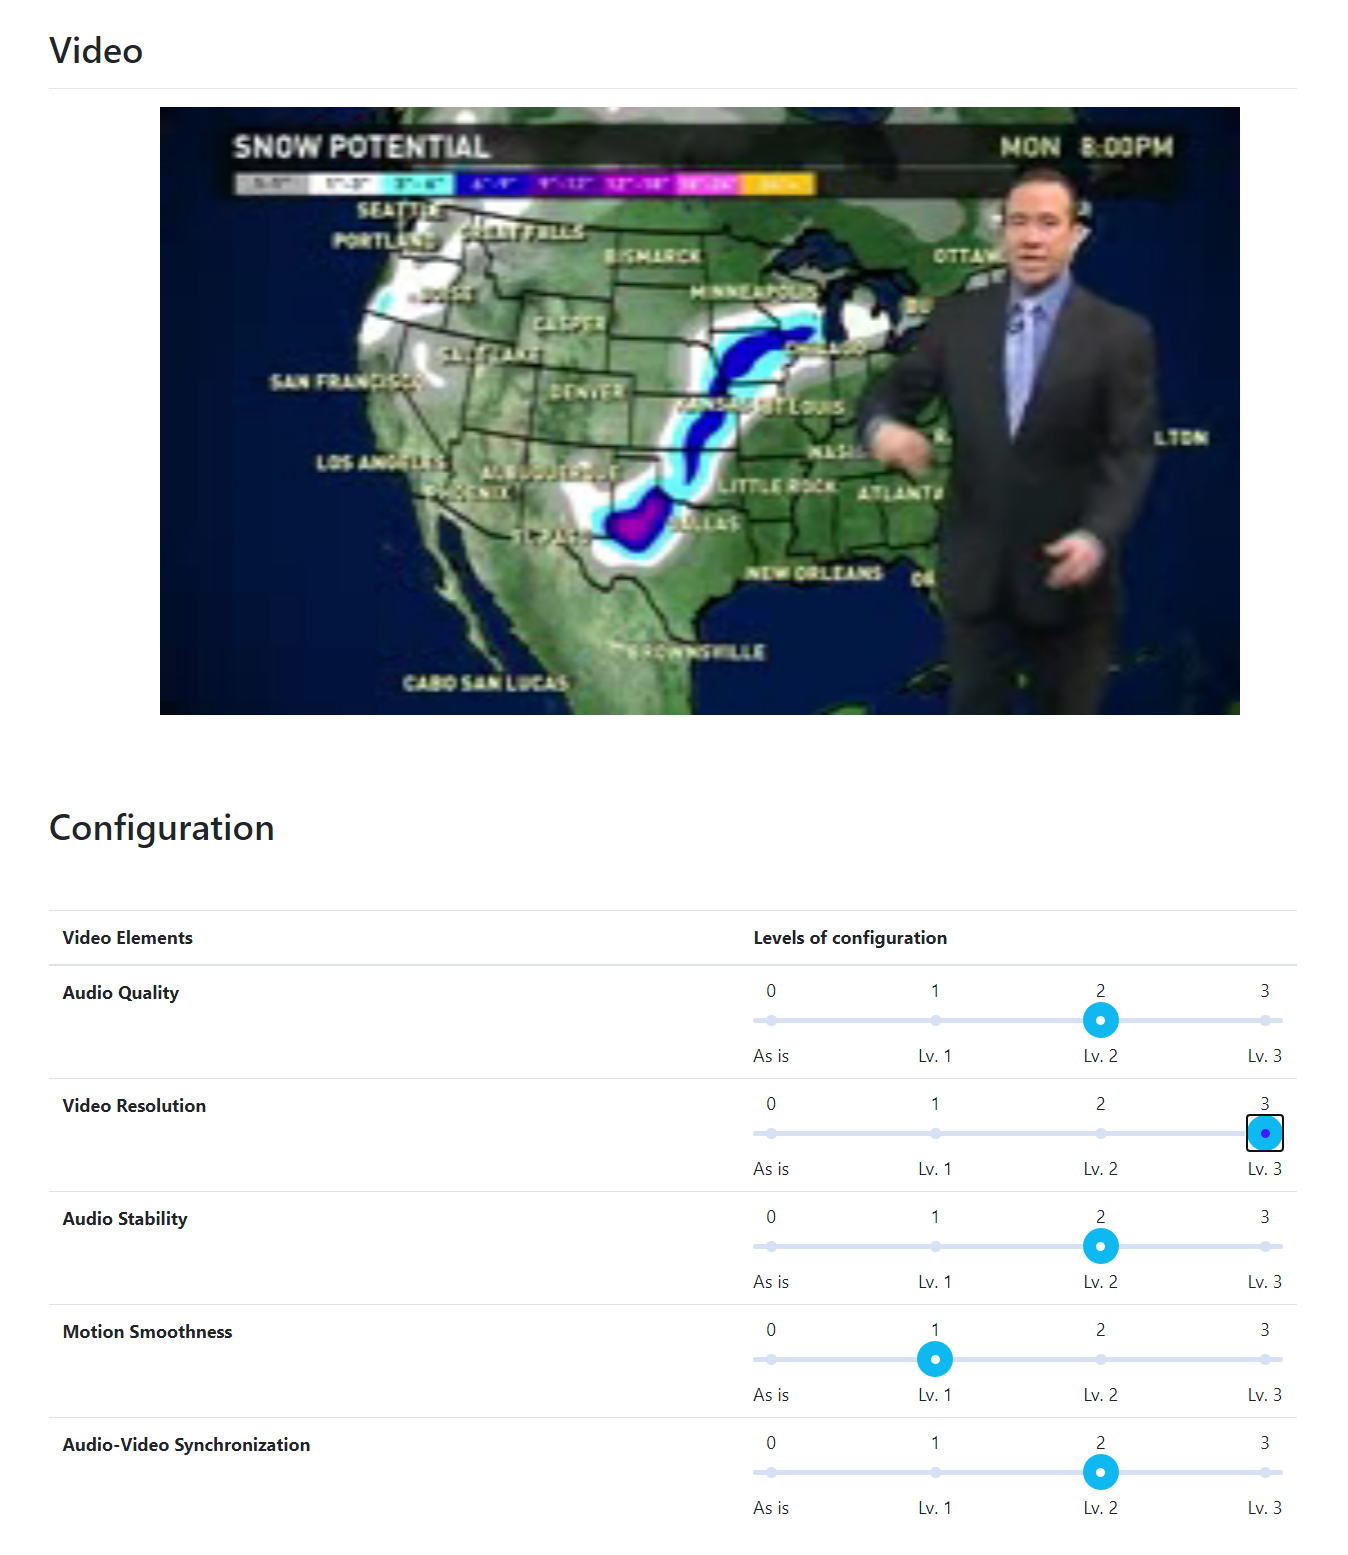
\includegraphics[width=0.8\textwidth, keepaspectratio=true]{content/image/video_playground.png}
    \caption{
        The Real-time Video Element Interface allows participants to adjust and understand how different video playback elements impact their viewing experience. We selected different levels for tech setting toggles according to prior research. The technical details of this implementation are included in the appendix.
    }
    \label{fig:exp2_playground}
\end{figure}


\subsubsection{Step 3. Video Playground}
To increase this experiment's fidelity, we introduced a fictional company to the participants, explaining that the goal is to ultimately provide a video-streaming product to the automotive industry using satellite-based Internet. We first showed participants the current prototype of the company's streaming service under limited bandwidth, which was a weather forecast video with all five elements at the worst quality in the range we designed to study\footnote{Motion smoothness: 32\% packet loss rate; Audio stability: 32\% packet loss rate; Video resolution: 210x280; Audio quality: 8kHz sampling rate; Audio-video synchronization: audio plays 2250ms ahead of the video}. After experiencing the current prototype, the participants moved on to the next page.

We then instructed them to explore how various enhancement levels on different elements in the current prototype would improve their viewing experience. To help them better understand the enhancements' impact, we built a video playground shown in Fig \ref{fig:exp2_playground}. This playground showed real-time changes in the video's overall quality as the participants adjust the control panel to a specific combination of different levels of enhancements for the five video elements. It is important to note that this interface is important because we asked participants to elicit preferences among the different \textit{perspectives} of the same subject matter. Each of these perspectives might not be independent of one another.

This interface showcased a weather forecast video on the top of the page. For each of the five video playback elements, we provided a slider with four levels of tickers. Participants can toggle any of these five elements to any of the four levels at any time. According to the quality levels the participants set, the video playback will immediately apply those changes. Participants can pause and play the video at any time, and they can replay the video as many times as they like. We encouraged participants to test out different combinations freely in this playground.

With Level 0 at the lowest quality and Level 4 at the highest, we designed the intermediate levels based on prior research \cite{claypool1999effects,oeldorf2012bad, noll1993wideband,knoche2008low, steinmetz1996human} such that the changes between each level of an element have a quasi-linear impact on viewers' perception. The five levels of the five video playback elements are listed below, from Level 0 to Level 3:
\begin{itemize}
    %20\%, 8\%, 4\%, and 0\%
    \item Motion Smoothness: 32\%, 20\%, 8\%, 4\%, and 0\%
    %20\%, 8\%, 4\%, and 0\%
    \item Audio Stability: 32\%, 20\%, 8\%, 4\%, and 0\%
    %210x280, 294x392, 364x486, and 420x560     
    \item Video Resolution: 210x280, 294x392, 364x486, 420x560, and 600x800 
    %8kHz, 11kHz, 16kHz, and 48kHz 
    \item Audio Quality: 8kHz, 11kHz, 16kHz, 48kHz, and 96kHz
    %1850, 1615, 1050, or 0 ms ahead
    \item Audio-Video Synchronization: 2250ms, 1850ms,  1615ms, 1050ms, or 0ms ahead
\end{itemize}

A text box was below this interface, asking participants to describe how changing the elements impacted their experience to make sure participants did toggle the settings.

\subsubsection{Step 4. Surveying Preferences}
After the participants were confident, they understood how the enhancements on different video playback elements would impact their viewing experience and complete the short question. We collected participants' feedback on how critical the improvements on each video element in the current prototype understand the weather forecast video's content. We divided all participants into two groups: the first group would complete the Likert survey first followed by a QV survey; the second group would complete the same two surveys in reverse order. The interface for Likert and QV are provided in the supplementary materials. The QV interface is similar to Figure \ref{fig:qv_donation}, for which each of the societal causes is now the five video elements. Unlike the previous experiment, we randomized the orders of each participant's options to prevent ordering effects. Our findings from experiment one allowed us to designed the credit budget to be 100 voice credits, derived from $N^2 x O$, where $N=5$ and $O=4$.

\subsubsection{Step 5. Distraction Survey}
Before moving on to the task that elicits the participant's underlying preference, we designed a distraction survey similar to experiment one. This survey prevents participants from translating their survey responses directly to the tasks that are to follow. We also told participants that this survey results would be used in a matching process for the next task. This survey asked participants' preferences across different subscription tiers for several well-known streaming services.

\subsubsection{Step 6. Design a Product}
Participants complete the experiment by designing a product. This task aims to capture a participant's actual underlying preferences on how critical they \textit{value} each of the five video elements. This is non-trivial, especially compared to our previous design using donations. We need to design a scenario and collect the behavioral data when participants are interacting with the task. We created the ``Design a Product'' task.

To create a high fidelity scenario, we told participants that the system distributed them into the designer group, who will design and assemble a streaming service for cars via satellite internet. Their goal is to design and price their product such that another participant, similar to them based on demographic information and the distraction survey from the buyers' group, would be willing to purchase the product. We emphasized to the participants that it is important to design the product such that it is affordable but allows the buyer to understand the weather forecast video's content.

The instruction also told participants to consider that each element is associated with a cost, and the buyer will need to pay each element's cost. We told participants that if the buyer decides to purchase the product, they will receive 10\% of the final price they proposed as their commission. 

There are two steps to guide participants to complete this task. We provided the interface for the two steps in Figure \ref{fig:exp2_store}. The first step starts by asking participants to select one of the two quality for each video element and ``assemble'' the product. In the second step, participants were asked to provide a price they think are reasonable to the five elements based on the qualities they selected. The sum of these price tags becomes the total price of the product. Participants were reminded throughout this task that the higher they priced the elements, the more their bonus could be. However, if they price the product too high, buyers might not purchase their design, and they would fail to gain any bonuses. 

Participants do not know that there does not exist a ``buyers'' group in this task. The goal of this design is to figure out the willingness-to-pay for each participant. One could view this task as a reverse auction, in which participants need to price how they value each of the elements according to their beliefs. If they price the product higher than their accurate valuations, this means that the ``buyer'' that is similar to them would reject their proposal, given the likely value the elements the same. Vice versa, if the participants set their prices lower than their belief, they lose out on potential opportunities to earn the bonuses. This made this task incentive-compatible. 

\begin{figure}[htpb]
    \centering
    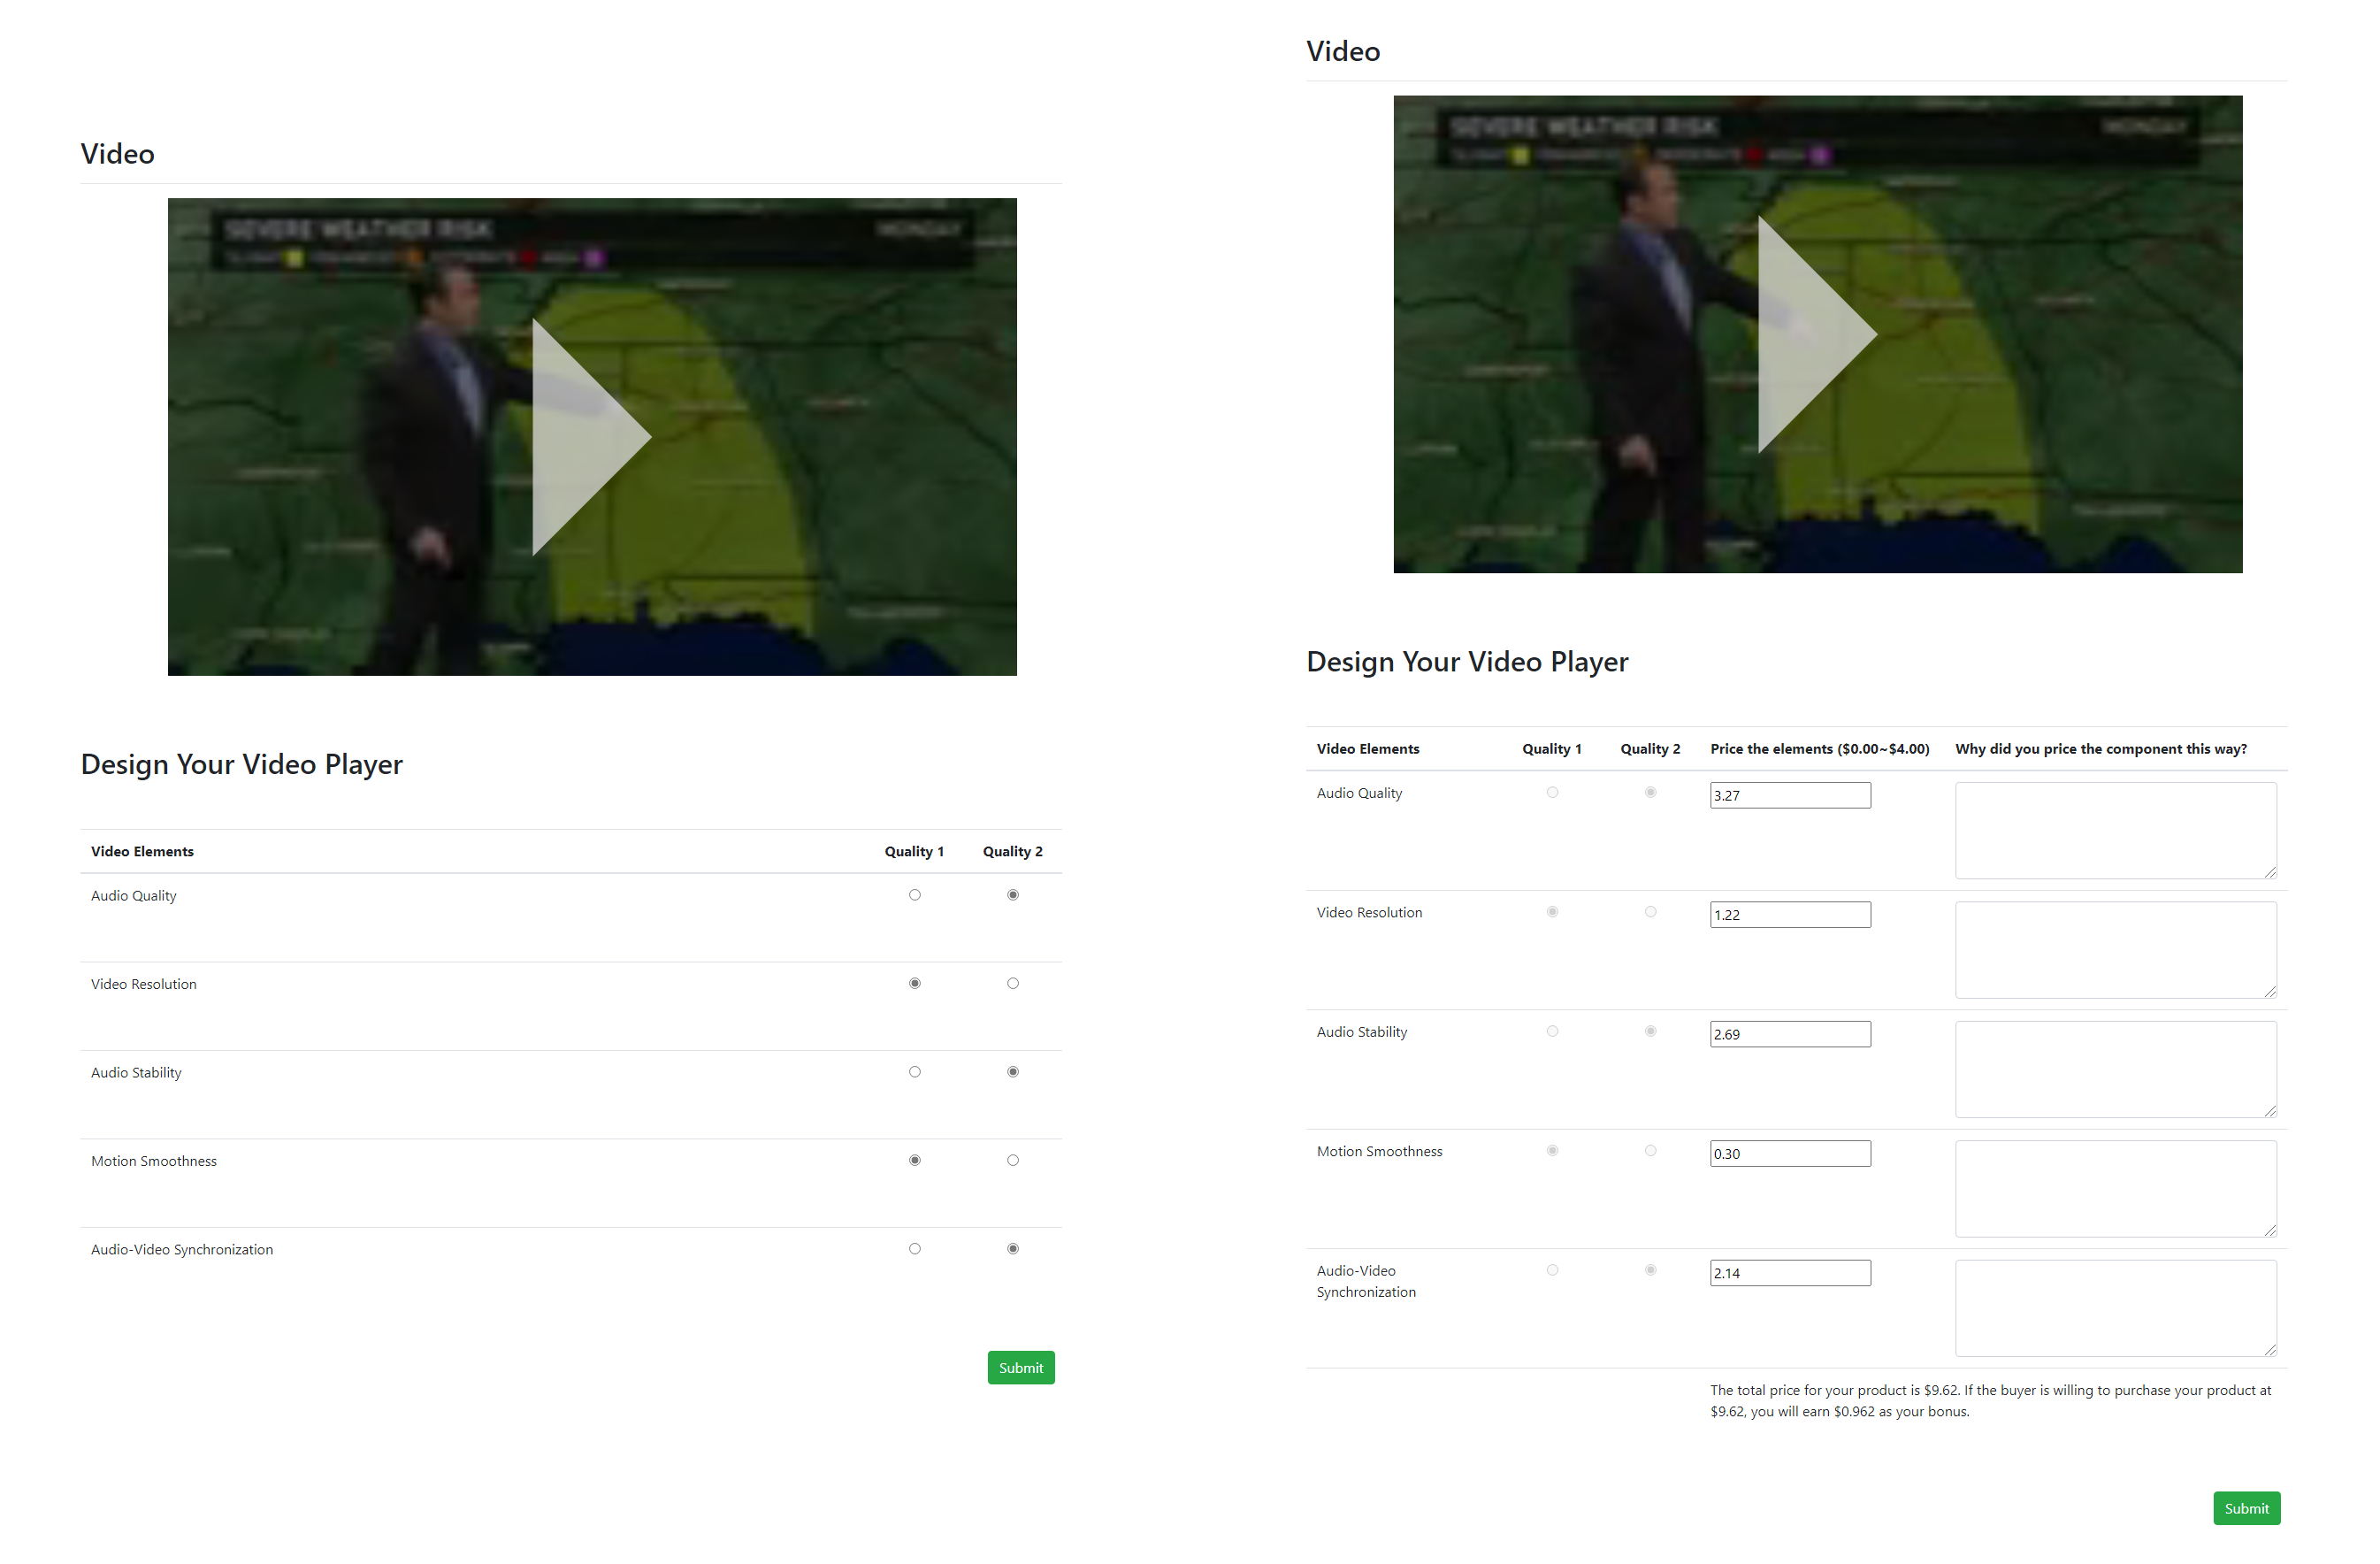
\includegraphics[width=\textwidth, keepaspectratio=true]{content/image/design_task.png}
    \caption{
        The two steps participants encounter when completing Step 6 of the survey. Participants would first need to elect the quality that they would involve into their video streaming product. Participants can see real time changes to the video as they select the combinations. Once they made their decision, participants would price each of the elements, each of them up to \$4 dollars. Participants would recieve a commission of 2\% based on some criteria.
    }
    \label{fig:exp2_store}
\end{figure}

Notice that instead of giving participants the power to select the quality over various levels as they did in the video playground in step three. We only provide two qualities for each video element. Quality one refers to level 0 in the playground, basically the worst one they had experienced. However, for quality 2, we designed the values to match prior research claiming that quality is the ``accepted level'' in their experiment\footnote{Place the five quality two values here}. This binary design prevents us from bounding participants' choices when provided a slider. Participants are essentially making a decision of whether a video element is ``important'' or ``not important.''

\subsection{System Design}
In this experiment, we build on top of the system for experiment one. To create real-time adjustments, we created the different qualities of video and audio files independently ahead of the experiment. When there is a change in the audio or video quality toggle, the system serves the correct combinations of video and audio files. JavaScript in the front-end was responsible for creating the video-audio synchronization.
This design balances the need for network speed, preventing from streaming every configuration from the server. It also prevents the need for a powerful client such that video and audio qualities were not computed directly on the client. The experiment source code for experiment two is publicly available \footnote{Not yet public}, and so is the video interface as a stand-alone repository \footnote{https://github.com/hank0982/QV-app}. More details are provided in the appendix.

\subsection{Analysis Method}

Since RQ2 is also about the degree of alignment, similar to RQ1, we followed a similar analysis approach as described in \Cref{method_exp1}. In experiment 2, we compared the alignment between survey responses with the prices set in an incentive-compatible scenario. We used the same definition of ``alignment" and the same metric for alignment, Cosine similarity angle, as explained in \Cref{alignment_metric}. For the Likert group, we mapped the ordinal responses into a vector where the result for each video element ranges from $-2$ to $2$. For QV, the vector contains the number of votes for each video element. Then, we computed the Cosine similarity angle between a Likert or QV vector and the absolute prices set by the same participant,.

Once we obtained the two sets of Cosine similarity angle, one for Likert and one for QV, we applied the same Bayesian formulation to model the mean Cosine similarity angle in both groups as detailed in \Cref{exp1:The Bayesian Model}. Then, we compared how different the two distributions were.